% Copyright 2021 Edoardo Riggio

% Licensed under the Apache License, Version 2.0 (the "License");
% you may not use this file except in compliance with the License.
% You may obtain a copy of the License at

% 	http://www.apache.org/licenses/LICENSE-2.0

% Unless required by applicable law or agreed to in writing, software
% distributed under the License is distributed on an "AS IS" BASIS,
% WITHOUT WARRANTIES OR CONDITIONS OF ANY KIND, either express or implied.
% See the License for the specific language governing permissions and
% limitations under the License.

\documentclass{article}

\usepackage{hyperref, amsmath, graphicx, amssymb, csquotes, listings}
\usepackage{fancyvrb,newverbs,xcolor}

\graphicspath{ {./assets/} }

\definecolor{cverbbg}{gray}{0.93}

\newenvironment{cverbatim}
 {\SaveVerbatim{cverb}}
 {\endSaveVerbatim
  \flushleft\fboxrule=0pt\fboxsep=.5em
  \colorbox{cverbbg}{\BUseVerbatim{cverb}}%
  \endflushleft
}

\newenvironment{lcverbatim}
 {\SaveVerbatim{cverb}}
 {\endSaveVerbatim
  \flushleft\fboxrule=0pt\fboxsep=.5em
  \colorbox{cverbbg}{%
    \makebox[\dimexpr\linewidth-2\fboxsep][l]{\BUseVerbatim{cverb}}%
  }
  \endflushleft
}

\newcommand{\ctexttt}[1]{\colorbox{cverbbg}{\texttt{#1}}}
\newverbcommand{\cverb}
  {\setbox\verbbox\hbox\bgroup}
  {\egroup\colorbox{cverbbg}{\box\verbbox}}
  
\lstdefinestyle{c++}{
  frame=single, language={C++}, numbers=left, numberstyle=\tiny, tabsize=4, breaklines=true,
  basicstyle=\ttfamily\scriptsize,
  keywordstyle=\color{blue}\ttfamily,
  otherkeywords={WIDTH},
  keywords=[2]{__shared__},
  keywordstyle=[2]\color{orange}\ttfamily,
  stringstyle=\color{red}\ttfamily,
  commentstyle=\color{green}\ttfamily
}

\begin{document}
\begin{titlepage}
    \begin{center}
        \vspace*{1cm}
        
        \Huge
        \textbf{Computer Graphics Cheatsheet}
        
        \vspace{0.5cm}
        \LARGE
        
        \vspace{.5cm}
        
        Edoardo Riggio
   		  \vspace{1.5cm}
       
        \vfill
        
        \today
        
        \vspace{.8cm}
          \Large
          Computer Graphics - SA. 2021 \\
        Computer Science\\
        Universit\`{a} della Svizzera Italiana, Lugano\\
        
    \end{center}
\end{titlepage}

\tableofcontents

\newpage

\section{Ray Tracing}
\textbf{Ray tracing} is a method of graphics rendering that simulates the physical behaviour of light.

\subsection{Whitted Ray Tracing}
One ray is traced for every single pixel. These are known as the \textbf{primary rays}. \\ \\
For each of the rays, we need to find their intersection with the scene. After we do so, secondary rays can be generated. Such rays are:

\begin{itemize}
	\item Shadow Ray
	\item Reflection Ray
	\item Refraction Ray
\end{itemize}
The color of each of the pixels is determined based on the aggregated color of the rays.

\begin{center}
	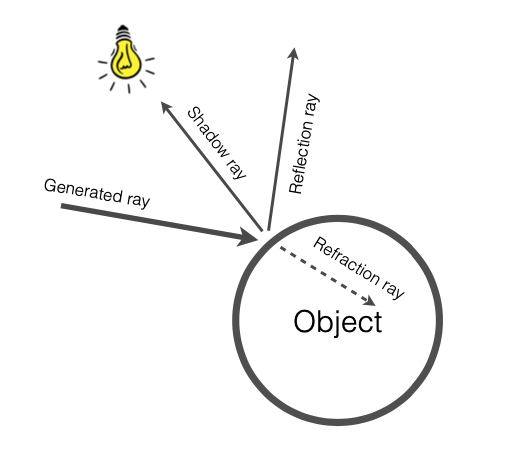
\includegraphics[width=5cm]{whitted_rt.png}
\end{center}
The secondary rays are recursively generated. Some termination conditions for this generation are:

\begin{itemize}
	\item Ray leaves the scene without ever hitting an object
	\item Maximal recursion depth is reached
	\item Contribution of the ray to the final color is negligible
\end{itemize}

\subsection{Camera / Image Definition}
We are considering a global coordinate system for the raytracer. Some of the characteristics of the \textbf{camera} are:

\begin{itemize}
	\item It is located at the origin $(0, 0, 0)$
	\item It has a horizontal opening $\alpha$, the FOV (Field Of View)
\end{itemize}
Some of the characteristics of the \textbf{image} are:

\begin{itemize}
	\item Image plane is located at $z = 1$
	\item Resolution of the image is of $w \cdot h$ pixels
	\item Pixels have indices $(i, j)$ and coordinates $p_{ij} = (x_{ij}, y_{ij}, z_{ij})$
\end{itemize}

\begin{center}
	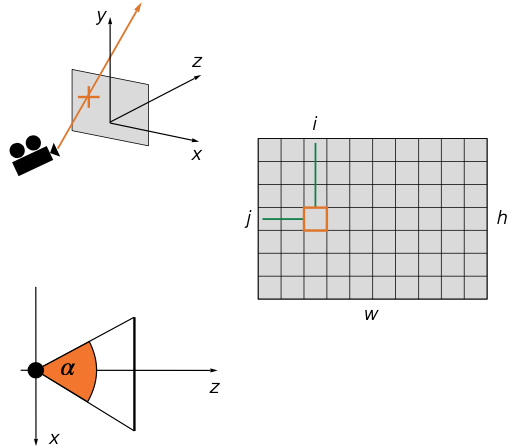
\includegraphics[width=6cm]{scene_def.png}
\end{center}

\subsection{Ray Computation}
The equation of a \textbf{ray} is the following:

\[ \gamma(t) = o + dt \] \\
Where $t$ is the distance between the origin and the intersection with an object, $o$ is the point representing the camera position, and $d$ is the vector representing the viewing direction -- of magnitude 1.

\begin{center}
	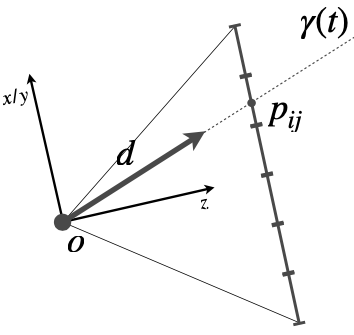
\includegraphics[width=5cm]{ray_comp.png}
\end{center} 
In order to compute the vector $d$, we need to do the following:

\begin{lstlisting}[style=c++]
s = (2 * tan(alpha / 2)) / 2;
X = (-w * s) / 2;
Y = (h * s) / 2;

for (int i = 0; i++; i < w) {
	for (int j = 0; j++; j < h) {
		dx = X + (i * s) + (0.5 * s);
		dy = Y - (j * s) - (0.5 * s);
		dz = 1;
		
		d = glm::vec3(dx, dy, dz);
		d = glm::vec3.normalize(d)
	}
}
\end{lstlisting}

\subsection{Ray-Sphere Intersection}
In order to define a \textbf{sphere}, we need to set the centre and the radius. Once that is done, we need to check is the sphere intersects with the generated ray. To do so we need to check if there is some $t$ such that:

\[ ||~\gamma(t) - c~|| = r \] \\
In order to find the $t$, we use the following procedure.

\begin{align*}
	a & = \langle c, d \rangle \\
	D & = \sqrt{||~c~||^2 - \langle c, d \rangle^2} \\
	t_{1,2} & = \langle c,d \rangle \pm \sqrt{r^2 - D^2}
\end{align*}
If the ray intersects the sphere and the camera is not inside of the sphere, then the pixel corresponding to the intersection is painted.

\section{Lighting Models}
In order to compute the color values on an object's surface we can use rules based on the laws of physics -- radiometry and photometry. These rules model the effect of:

\begin{itemize}
	\item \textbf{Light Sources}
	\vspace{.2cm} \\
	Position, intensity and colour.
	
	\item \textbf{Object Surface}
	\vspace{.2cm} \\
	Geometry and reflective properties.
\end{itemize}

\subsection{Illumination Factors}
The intensity of a color depends on several different factors:

\begin{itemize}
	\item The colour and reflective properties of the object
	\item The position and intensity of the light sources
	\item The position of the viewer
	\item The normal of the surface at point $p$
	\item The distance of point $p$ to the light source
\end{itemize}

\subsection{Components of the Phong Lighting Model}
These components are the \textbf{diffuse reflection}, the \textbf{ambient illumination}, and the \textbf{specular highlight}.

\subsubsection{Diffuse Reflection}
This type of reflection simulates Lambertian surfaces -- i.e. matte surfaces. Here the reflected light is dispersed evenly in all directions. \\ \\
There is also a material-dependent reflection constant $\rho_d \leq 1$. This is called the \textbf{diffuse coefficient}.

\begin{center}
	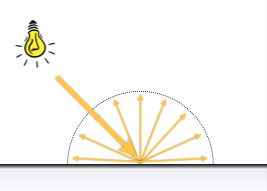
\includegraphics[width=4cm]{lambertian_surf.png}
\end{center}
The intensity $I_d$ of a surface coming from the diffuse reflection is proportional to the cosine of the angle between the surface normal $n$ and the direction of the light source $l$. This is known as the \textbf{Lambertian Cosine Rule}.

\begin{center}
	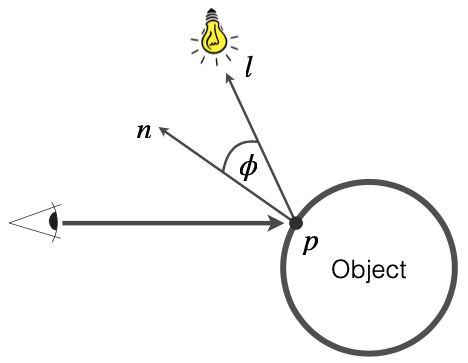
\includegraphics[width=5cm]{cos_rule.png}
\end{center}
The proper computation of the diffuse reflection is the following -- in which the Cosine Rule is applied:

\begin{align*}
	I_d &= \rho_d \cdot \cos\phi \cdot I \\
	&= \rho_d \cdot \langle n, l \rangle \cdot I
\end{align*}
Where $\rho_d$ is the diffuse coefficient, $n$ is the normal of the surface at point $p$, $l$ is the vector pointing towards the light source, and $I$ is the intensity of the light. \\ \\
An important thing to always check is that $\langle n, l \rangle > 0$.

\subsubsection{Ambient Illumination}
Ambient illumination is used in order to simulate indirect lighting. This refers to the effect of multiple inter-reflections of light between all objects, and to the isotropy and independence of light sources and viewpoints. \\ \\
There is a global constant $I$, and a material-dependent reflection constant $\rho_a \leq 1$. This is called the \textbf{ambient coefficient}. \\ \\
The ambient illumination is given by the following formula:

\[ I_a = \rho_a \cdot I \] \\
Where $\rho_a$ is the ambient coefficient, and $I$ is the intensity of the ambient lighting.

\subsubsection{Specular Reflection}
Specular reflection is used in order to simulate shiny surfaces. The incoming light is reflected in exactly one reflect direction. \\ \\
The specular reflection makes use of something known as the reflection vector.

\begin{center}
	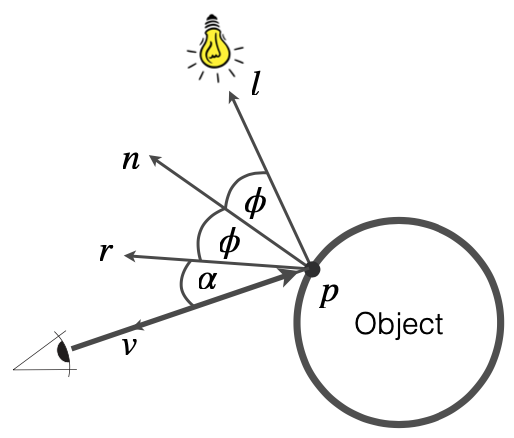
\includegraphics[width=5cm]{specular_refl.png}
\end{center}
The proper formulation of the specular reflection is the following:

\[ I_s = \rho_s \cdot \langle r, v \rangle^k \cdot I \] \\
Where $\rho_s$ is the specular coefficient of the object, $r$ is the reflection ray given by:

\[ r = 2n \cdot \langle n, l \rangle - l \] \\
Furthermore, $v$ is the viewing direction of the camera, $k \geq 1$ is the shininess coefficient, and $I$ is the light intensity.

\subsection{Phong Lighting Model}
The Phong lighting model is given by the superposition of ambient, diffuse, and specular terms for each light source. The final formula is the following:

\[ I = I_e + \rho_a \cdot I_a + \sum^n_{j = 1} (\rho_d \cdot \langle n, l_j \rangle + \rho_s \cdot \langle r_j, v \rangle^k) \cdot I_j \] \\
Where $I_e$ is the self-emitting intensity, $\rho_a$ is the diffuse coefficient, $I_a$ is the ambient intensity, $\rho_d$ is the diffuse coefficient, $n$ is the normal vector, $l$ is the vector pointing to the light source, $\rho_s$ is the specular coefficient, $r$ is the reflection ray, $v$ is the direction vector, $k$ is the shininess, and $I_j$ is the intensity of the $j$-th light source.

\subsection{Blinn-Phong Specular Reflection}
Here we use $h$ instead of $r$ in order to compute the specular reflection of an object.

\begin{center}
	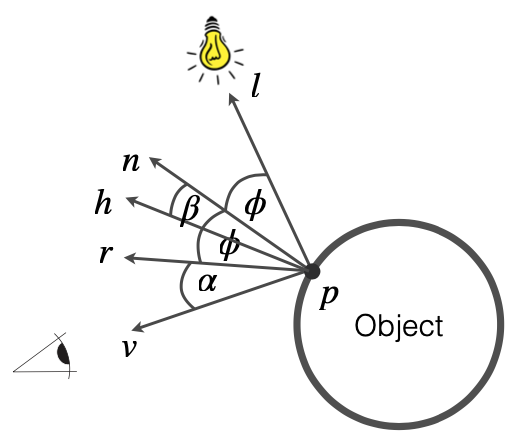
\includegraphics[width=5cm]{blinn_phong.png}
\end{center}
The proper formulation of the Blinn-Phong specular reflection is the following:

\[ I_s = \rho_s \cdot \langle n, h \rangle^{4k} \cdot I \] \\
Where $\rho_s$ is the specular coefficient, $n$ is the normal, $k$ is the shininess coefficient, $I$ is the light intensity, and $h$ is defined as:

\[ \frac{1}{2}(l + v) \] \\
Where $l$ is the light vector, and $v$ is the viewing direction.

\subsection{Light Sources}
\subsubsection{Point Light Sources}
\textbf{Point light sources} are a type of source that is isotropic -- radiates evenly in all directions, it is specified by a position, and has intensity $I$. \\ \\
\textbf{Directional light sources} are a special case of light sources which are only specified by direction. This is because it is an infinite set of rays that all have the same direction.

\subsubsection{Spot Light Sources}
This type of light source generates a light cone in a specified direction. In order to define the spot light source, we need to specify its position $p$, its direction $d$, and its opening angle $\Theta_L$.\\ \\
The intensity of the light is either maximal in the direction of $d$, or decreases following the formula:

\[ I'(\Theta) = \cos^k\Theta \cdot I \] \\
And it's 0 when $\Theta > \Theta_L$.

\subsection{Distance Attenuation}
The more the object is distant from the light source, the less it will be illuminated by the source. Its formal definition is:

\[ att(r) = \frac{1}{a_1 + a_2r + a_3r^2} \] \\
Where $r$ is the ray of light, and $a_1$, $a_2$, and $a_3$ are constant values.

\end{document}






























 
